\subsection{Performance analysis}
The performance of the six different functions resulting from the possibilities of permuting mnk are tested with square matrices with memory footprints ranging from a few kB to hundreds of MB. The results are seen in figure \ref{fig:permGraph_none} with no compiler options. All six permutations perform equally well when the memory footprint is less than the L2 cache. For memory footprints larger than L2, the permutations with the loop over $n$ maintain the same performance, while the other four permutations have a significant reduction of performance. This is due to the fact that $m$ is the row index for matrices B and C, and that works well with the C language which is row major, meaning that the caches lines go along the rows of the matrices. The performance does not degrade after exceeding L3 which shows that program does not utilize the caches optimally. If that was the case, the smaller bandwidth between the memory and the processor would cause a significant drop in the performance when the memory footprint exceeds L3.
\begin{figure}
\centering
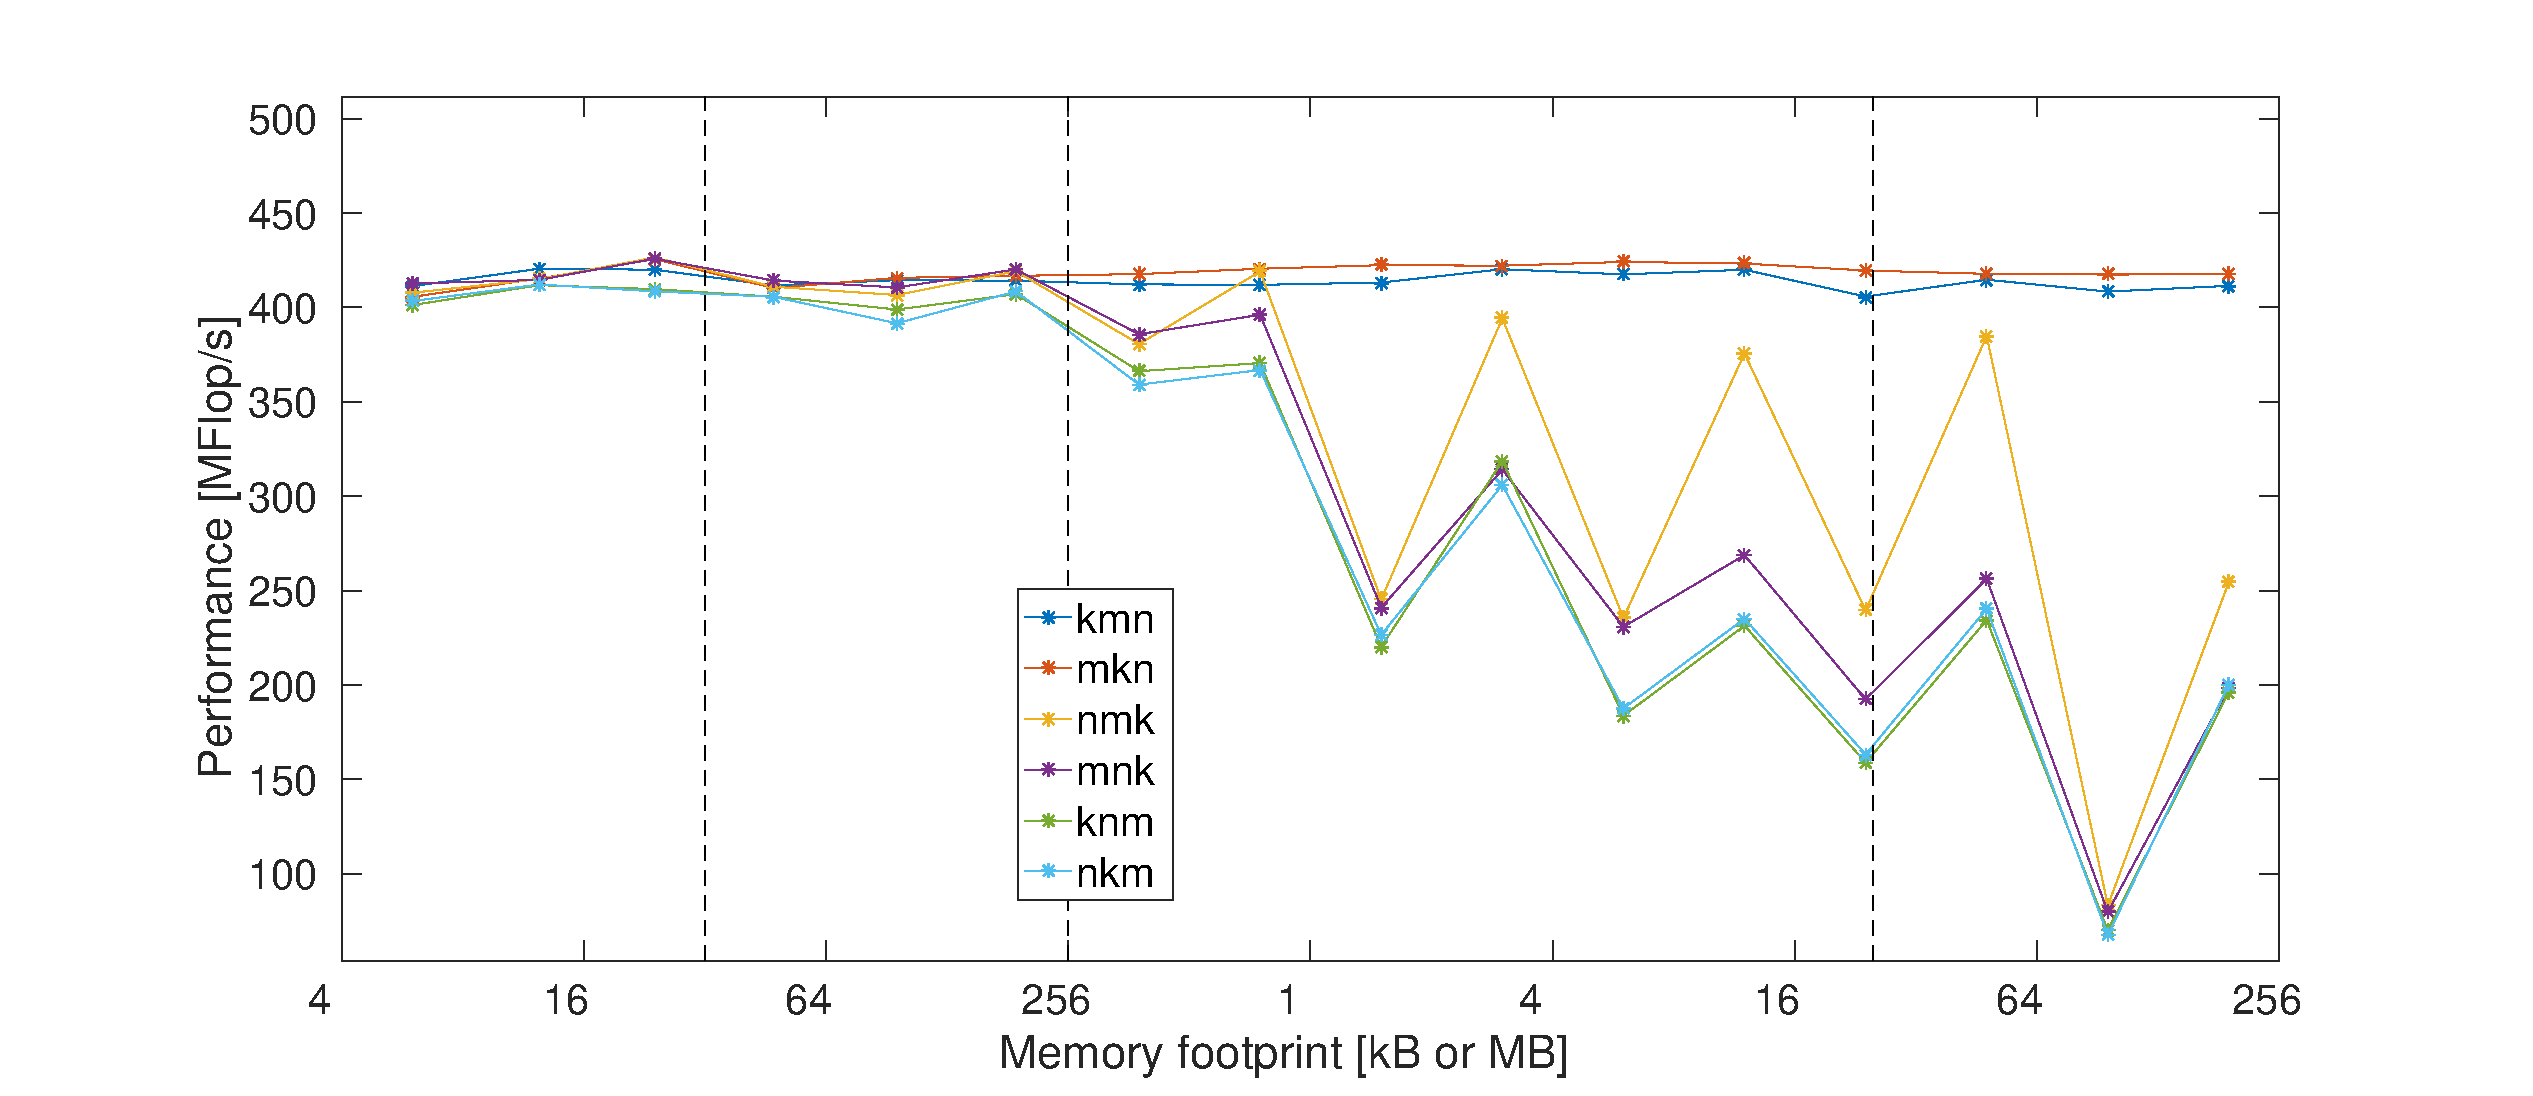
\includegraphics[width = 1.1\textwidth]{fig/permGraph_none.eps}
\caption{The performance of the different permutations versus the memory footprint, with L1, L2, and L3 caches shown as the vertical black dotted lines.}
\label{fig:permGraph_none}
\end{figure}
To investigate this, the same graph is produced, but this time the $\mathrm{-fast}$ option is activated in the Sun Studio compiler, and the results are shown in figure \ref{fig:permGraph_fast}. All six functions have improved performance compared to the case without compiler options, but the functions with $k$ as the inner loop, are a factor of $\sim 2$  slower for memory footprints which fit in either L1 and L2 caches. This is due to the fact that when $k$ is the inner loop, the program needs to fetch two new values to multiply together, and the compiler optimizer apparently has some issues optimizing this. When the memory footprint exceeds L2, the functions with $m$ as the inner loop drop off to the level of the functions with $k$ as the inner loop. This is because $m$ is the column size of matrices A and C, and looping over this as the inner loop goes against the row major format of C. For smaller memory footprints, the compiler is able to mitigate this issue, but after L2, the compiler optimizer can not fix the issue, and the performance drops. When the memory footprint does not exceed the size of the L3 cache, the performance of the functions with $n$ perform at a constant rate. This is again due to the row major format of C and $n$ being the row size of matrices B and C. After the L3 cahce size, the performance drops $\sim 10 \%$, which is less than expected, but that is probably due some extensive prefetching performed by the compiler when the $\mathrm{-fast}$ option is enabled. It is also worth noting that mkn performs better than kmn for all memory footprints, and the reason here is that the loop over $m$ is the slowest, and thus to achieve the best performance, this loop must placed as the outmost loop.

\begin{figure}
\centering
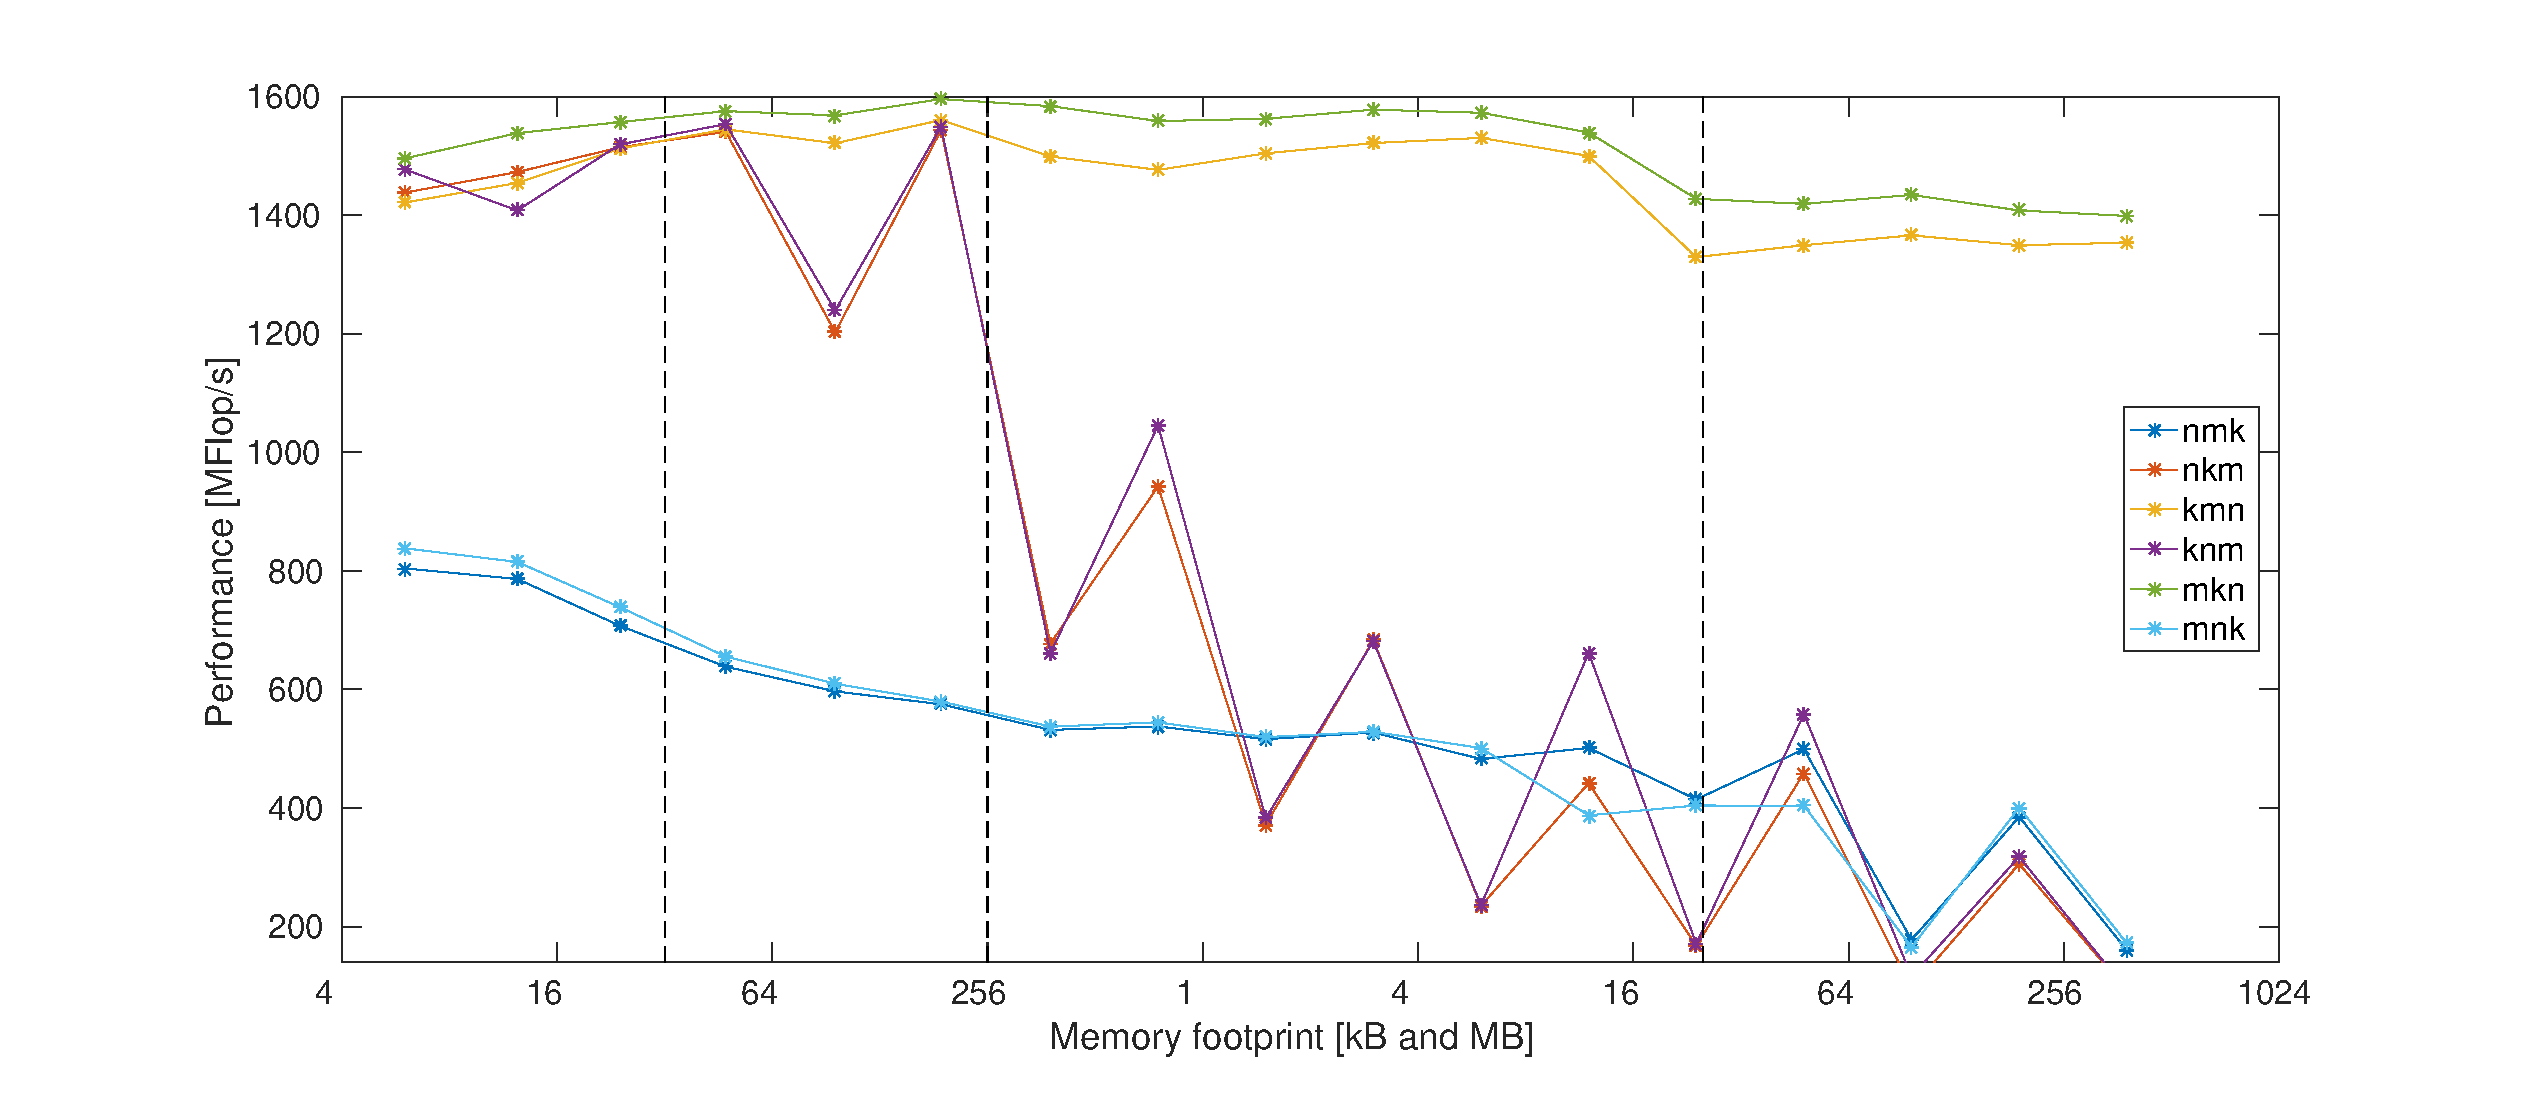
\includegraphics[width = 1.1\textwidth]{fig/permGraph_fast.eps}
\caption{The performance of the different permutations versus the memory footprint with compiler option $\mathrm{-fast}$ activated. L1, L2, and L3 caches shown as the vertical black dotted lines.}
\label{fig:permGraph_fast}
\end{figure}

One function prom each pair sharing the same inner loop is selected to investigate the effect of the different compiler options on the performance. Three options are chosen: General optimization -xO5, loop unrolling -unroll=8, and prefetching -xprefetch\_level=3. The three plots are seen in figure \ref{fig:compGraph}. As seen, neither prefetching nor unrolling does anything measureable to the performance, while -xO5 is responsible for the entire performance increase from the -fast option. We expected a performance increase from the unrolling because the code only specifies one multiplication per loop, and unrolling should decrease the relative amount of overhead calculations, thus increasing the performance even for small memory footprints, but it is not observed. This could be because the hard-coded unrolling value is not optimal for all matrix sizes, and thus it does not give a performance increase. The -fast option does unrolling, but probably with more dynamically. The prefetching was expected to give an increased performance for memory footprints exceeding the L3 cache, but that is not observed either, again most likely due to something else being the bottleneck, as is also evident from the fact that performance with no options is more or less constant for all memory footprints tested here.

In conclusion, the compiler optimizations can, for the right loop order, increase the performance by a factor of 4, but it was not possible to observe the effect from the individual options enabled alone.

\begin{figure}
\centering
\begin{subfigure}{1\textwidth}
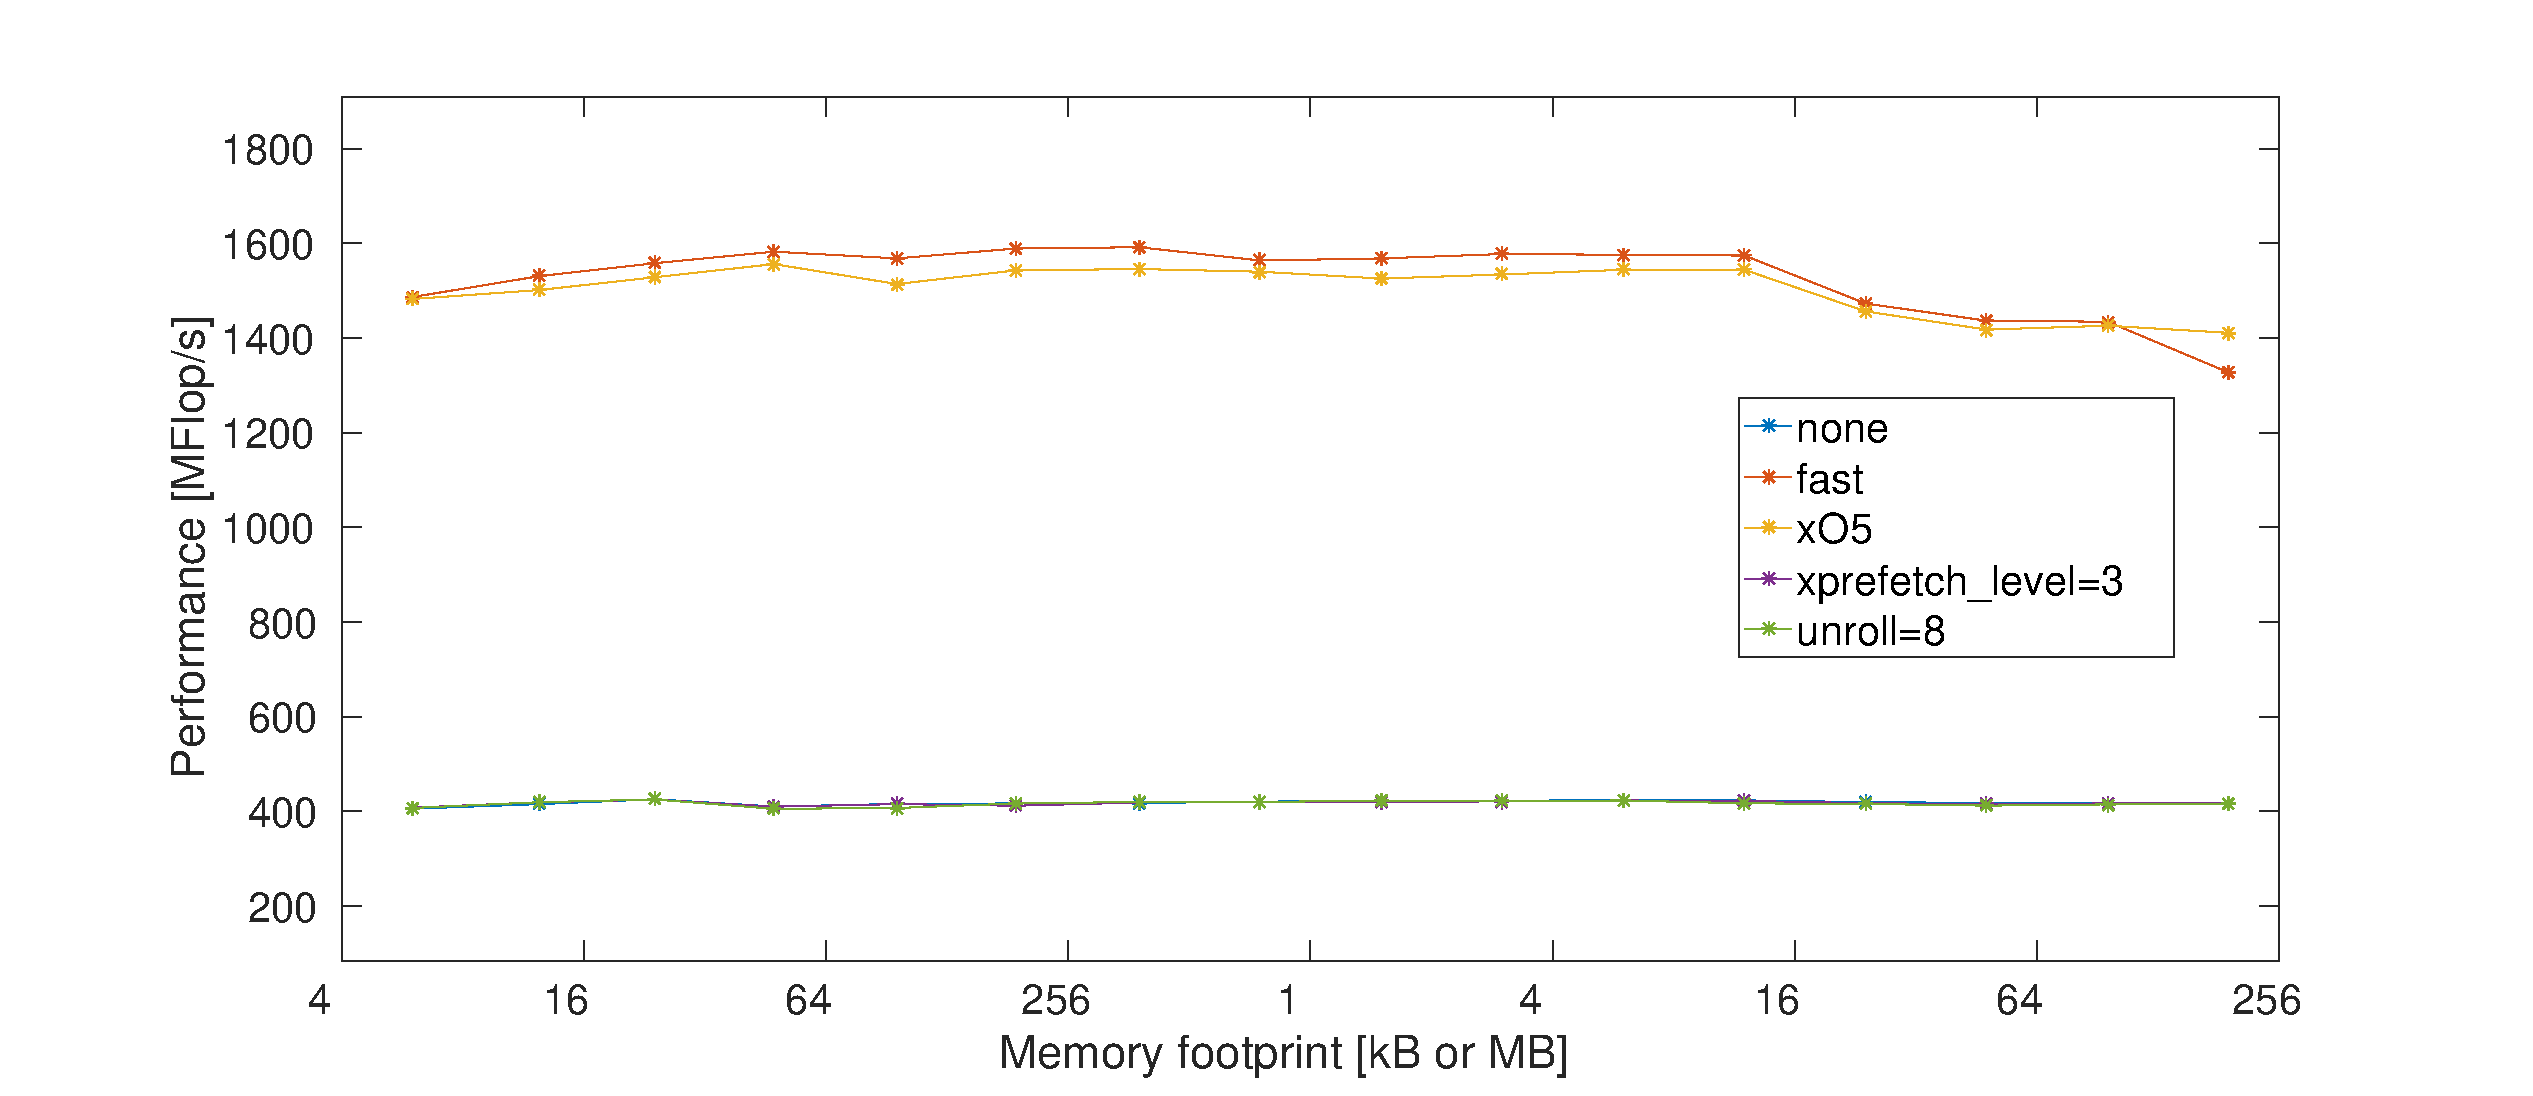
\includegraphics[width = \textwidth]{fig/compGraph_mkn.eps}
\caption{}
\label{fig:compGraph_mkn}
\end{subfigure}

\begin{subfigure}{1\textwidth}
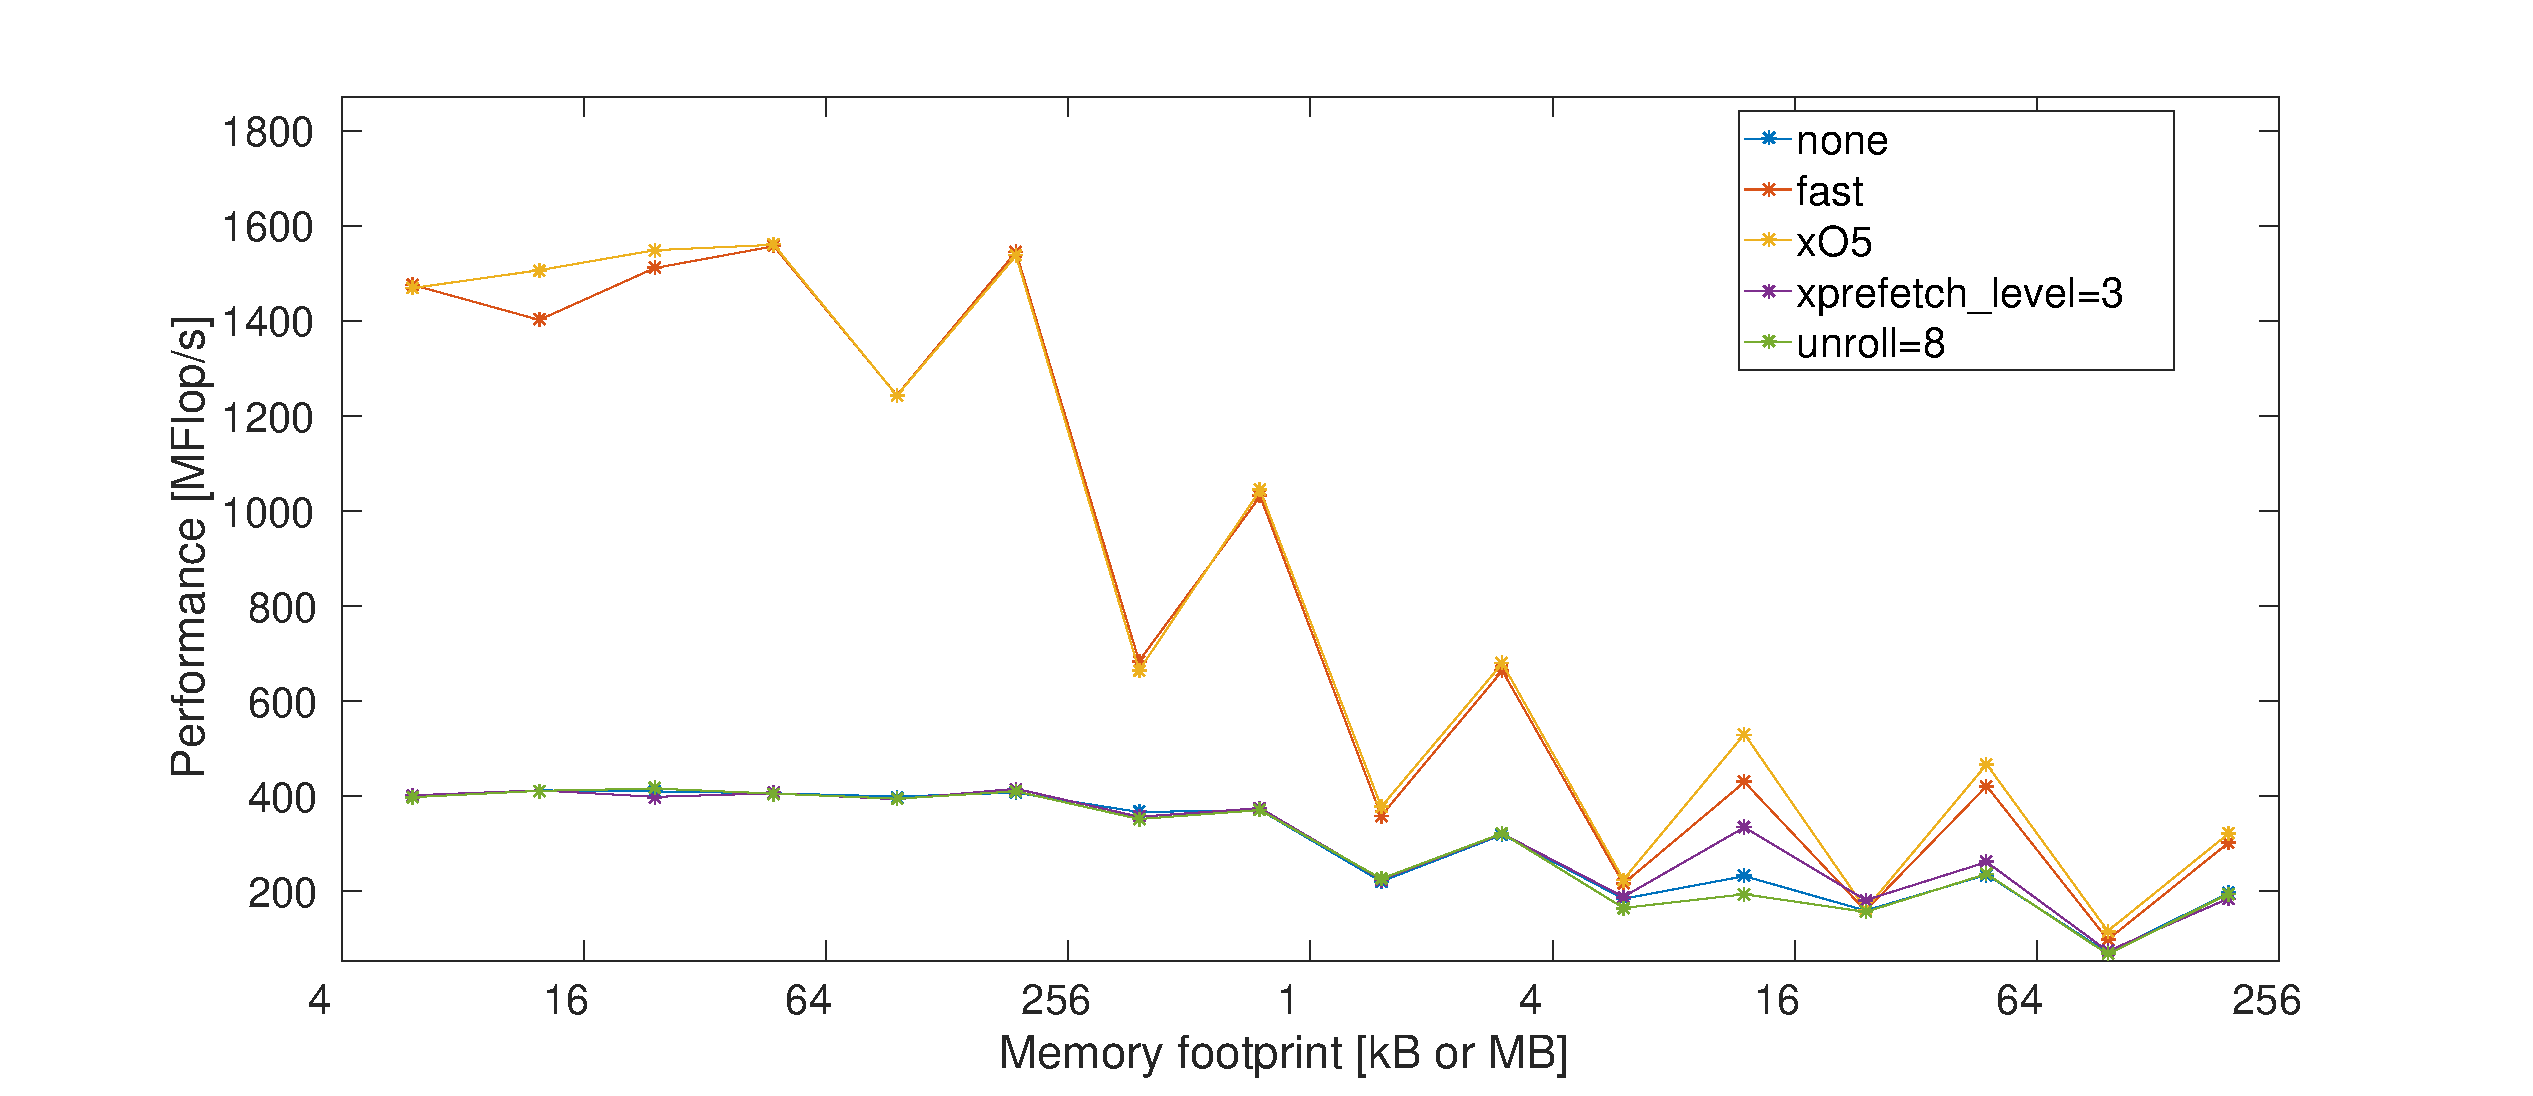
\includegraphics[width = \textwidth]{fig/compGraph_knm.eps}
\caption{}
\label{fig:compGraph_knm}
\end{subfigure}

\begin{subfigure}{1\textwidth}
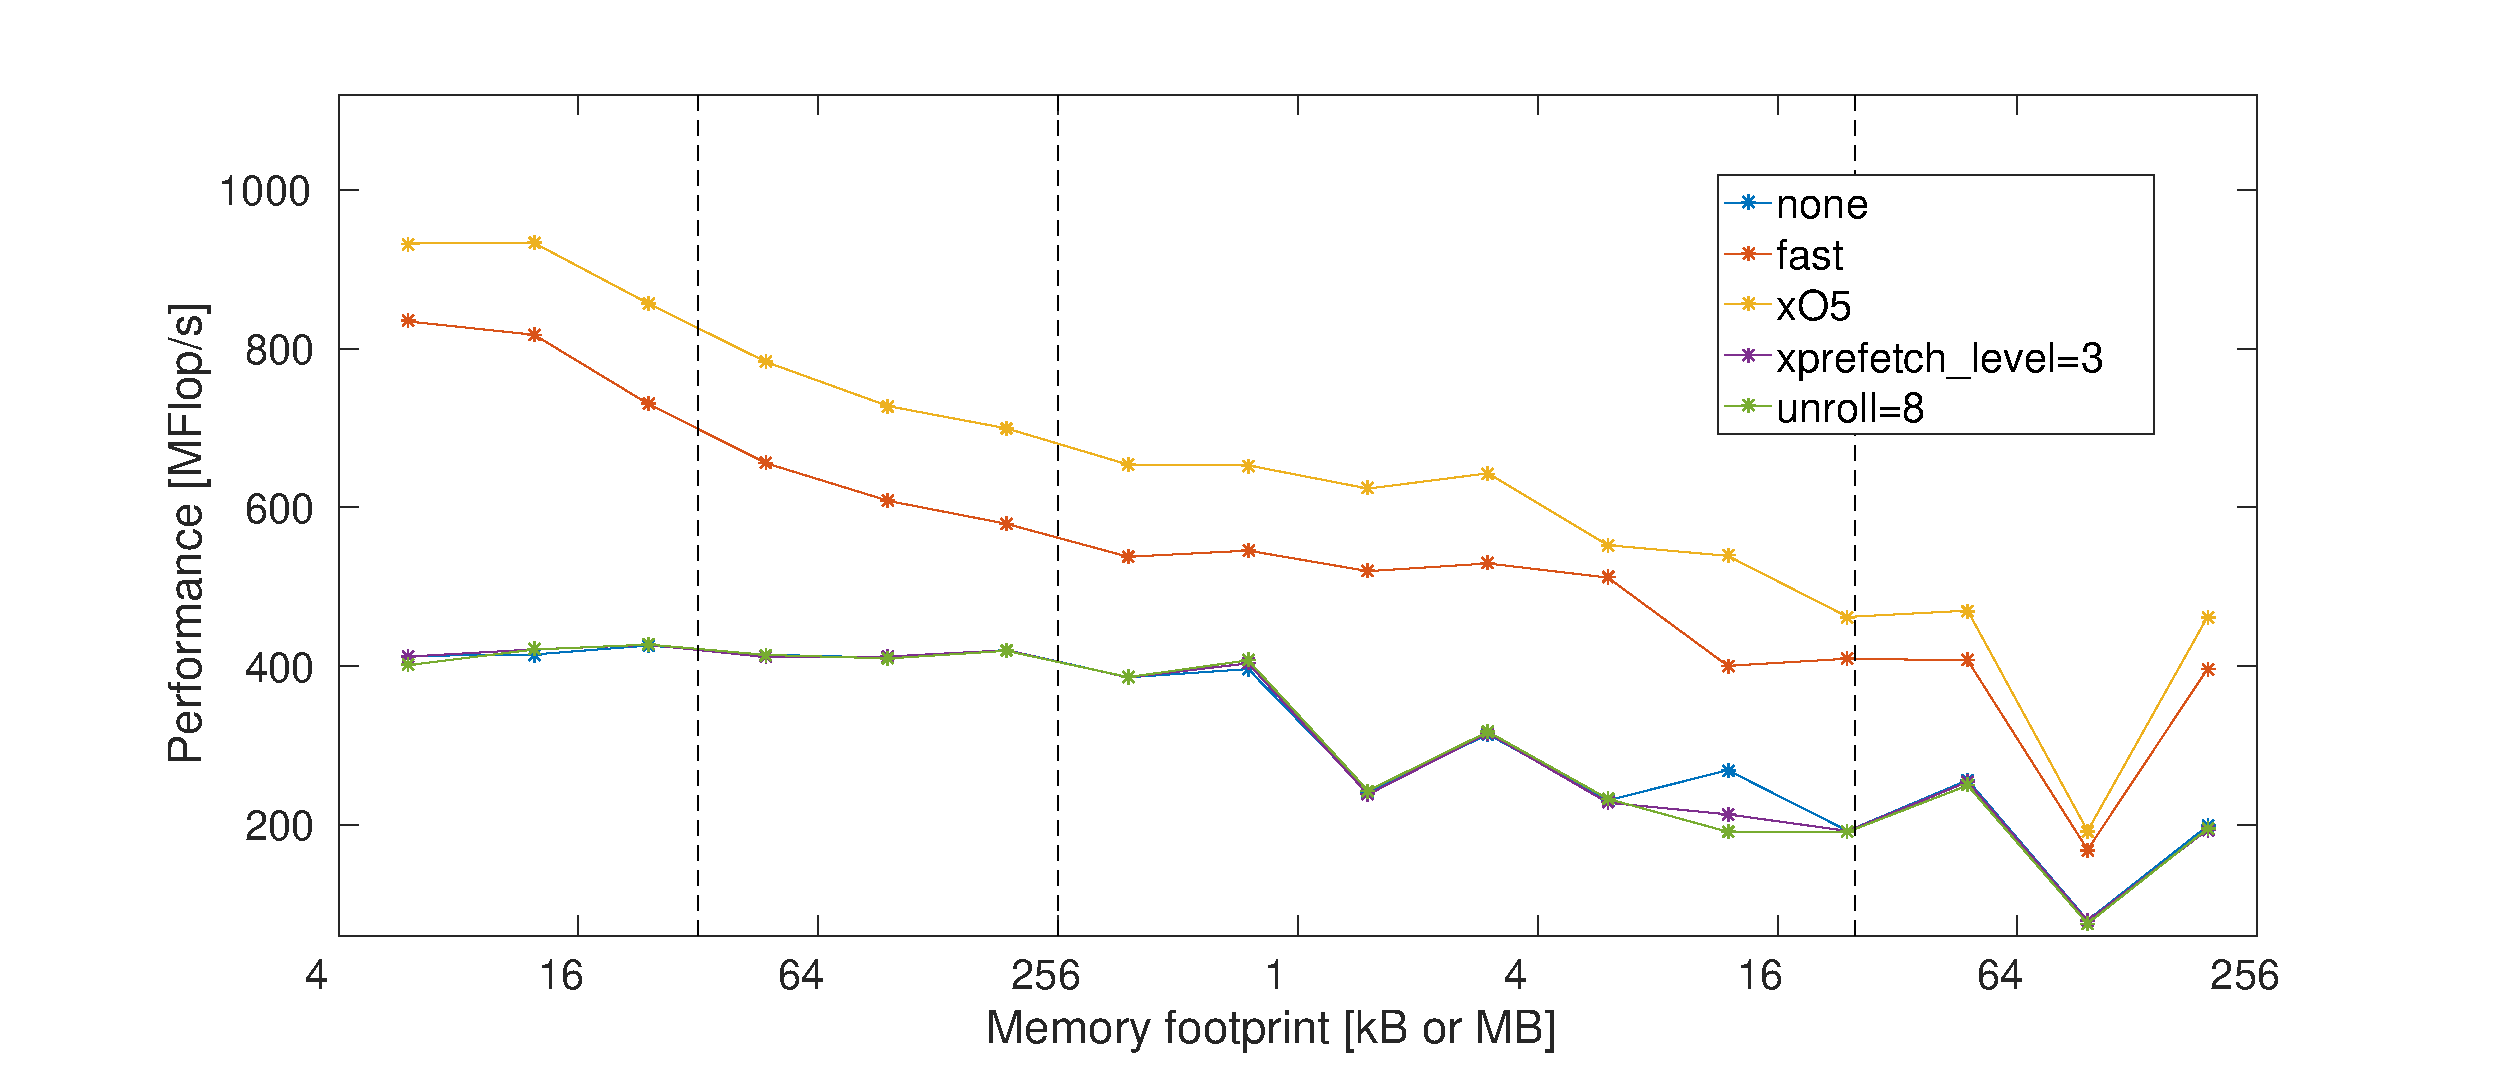
\includegraphics[width = \textwidth]{fig/compGraph_mnk.eps}
\caption{}
\label{fig:compGraph_mnk}
\end{subfigure}
\caption{Performance versus memory footprint with different compiler options for (\subref{fig:compGraph_mkn}) mkn, (\subref{fig:compGraph_knm}) knm, and (\subref{fig:compGraph_mnk}) mnk.}
\label{fig:compGraph}
\end{figure}


